\documentclass[12pt]{report}

\usepackage[utf8]{inputenc}
\usepackage[T1]{fontenc}
\usepackage{lmodern}
\usepackage[catalan]{babel}
\usepackage{geometry}
\usepackage{hyperref}
\usepackage{xcolor}
\usepackage{booktabs}
\usepackage[catalan]{todonotes}
\usepackage[bf,sf,small, pagestyles]{titlesec} % Format dels títols de secció
\usepackage[font={footnotesize, sf}, labelfont=bf]{caption} % Format dels peus de figura
\usepackage{graphicx}
\usepackage{amsmath, amssymb, xfrac}
\usepackage{siunitx}
\usepackage[catalan]{cleveref}

% Marges, etc
\geometry{
	a4paper,
	right = 2.5cm,
	left = 2.5cm,
	bottom = 3cm,
	top = 3cm,
	columnsep = 1cm,
	twoside
}
\setlength{\parskip}{0pt}
% Referències
\hypersetup{
	colorlinks,
	linkcolor = {red!50!blue},
	linktoc = page
}
\crefname{figure}{figura}{figures}

% Figures
\graphicspath{{./informe-2/figs/} {./informe-7/figs/} {./annexos/figs/}}

% Peus de pàgina
\newpagestyle{pagina}{
	\headrule
	\sethead*{}{}{\sffamily {\slshape Informe \thechapter: }\chaptertitle}
	\footrule
	\setfoot*{}{}{\sffamily \thepage}
}
\renewpagestyle{plain}{
	\footrule
	\setfoot*{}{}{\sffamily \thepage}
}
\pagestyle{pagina}

% Format del títol
\titleformat{\chapter}[display]{\centering \bfseries \sffamily \LARGE}{\large \sf Informe \thechapter}{4pt}{}{\thispagestyle{pagina}}
\titlespacing{\chapter}{0pt}{*2}{*4}

% Unitats
\sisetup{
	inter-unit-product = \ensuremath{ \cdot },
	allow-number-unit-breaks = true,
	detect-family = true,
	list-final-separator = { i },
	list-units = single
}
% Valor amb incertesa
\newcommand{\data}[3]{\SI[separate-uncertainty = true]{#1 \pm #2}{#3}}

% Format de l'abstract
\newlength{\currentparindent}
\newenvironment{resum} 
{ \setlength{\currentparindent}{\parindent} \noindent \begin{center} \begin{minipage}{0.8\linewidth} \setlength{\parindent}{\currentparindent} \footnotesize \slshape }
{ \end{minipage} \end{center}	\vspace{0.5cm} }

% Títol
\title{\sffamily \bfseries Laboratori d'Electromagnetisme}
\author{\sffamily Sandro Barissi, Adrià Marín, Arnau Mas, Robert Prat} 
\date{\sffamily 2018}

% Arxius a incloure
\includeonly{./informe-7/informe-7}

\begin{document}
\maketitle

\newpage
{\sffamily \tableofcontents}
\addcontentsline{toc}{part}{Informes}

% Informes
% Informe 2
\chapter{Força entre corrents}
\begin{resum}
	Aquest informe presenta els resultats de l'estudi de la força exercida entre dos corrents paral·lels pels quals hi circula la mateixa intensitat. Concretament, s'ha provat experimentalment la dependència lineal entre la força i el quadrat de la intensitat i entre la força i l'invers de la distància entre els fils.

	A més, s'ha trobat experimentalment el valor de la constant \( \mu_0 \) a partir de la llei de Biot-Savart, \( \mu_0 = \data{1.25}{0.04e-6}{N.A^{-2}} \) i \( \mu_0 = \data{3.0}{0.4d-6}{N.A^{-2}} \). El primer valor és consistent amb el tabulat, mentre que el segon només n'és de l'ordre. 

	Finalment, s'ha mesurat la component radial del camp magnètic terrestre, obtenint un valor de \( B = \data{1.59}{0.18d-5}{T} \) de l'ordre del que descriuen altres articles.
\end{resum}

\begin{multicols*}{2}
	\section{Introducció i Objectius}
	Quan un fil de longitud \( L \) pel qual hi passa un corrent \( I \) és sotmès a un camp magnètic uniforme de mòdul \( B \) experimenta una força proporcional a aquestes tres quantitats i perpendicular tant al fil com al camp magnètic. És a dir
	\begin{equation} \label{eq:forca magnetica} 
		F = BIL.
	\end{equation}
	En particular, com que el camp magnètic a distància \( r \) un fil d'aquestes característiques és, en bona aproximació si \( L \ll r \) és
	\begin{equation*}
		B = \frac{\mu_0 I}{2\pi r},
	\end{equation*}
	deduïm que la força entre dos cables paral·lels pels quals i passa corrent en el mateix sentit és atractiva i val
	\begin{equation} \label{eq:forca i corrent}
		F = \frac{\mu_0I^2L}{2\pi r}.
	\end{equation}

	L'objectiu principal d'aquesta pràctica és avaluar experimentalment aquestes relacions. És a dir, s'han fet mesures de la força entre dos fils a diferents corrents i separacions amb l'objectiu d'observar les relacions \( F \propto I^2 \) i \( F \propto r^{-1} \). A més, amb aquestes mesures es pot donar un valor de la constant \( \mu_0 \).  

	Finalment també s'ha pogut mesurar el valor de la component radial del camp magnètic terrestre. 

	\section{Mètode experimental}
	Totes les mesures s'han pres en una balança de corrents. La \cref{fig:balanca} mostra un esquema del dispositiu, amb els elements principals.
	\begin{figure*}
		\centering
		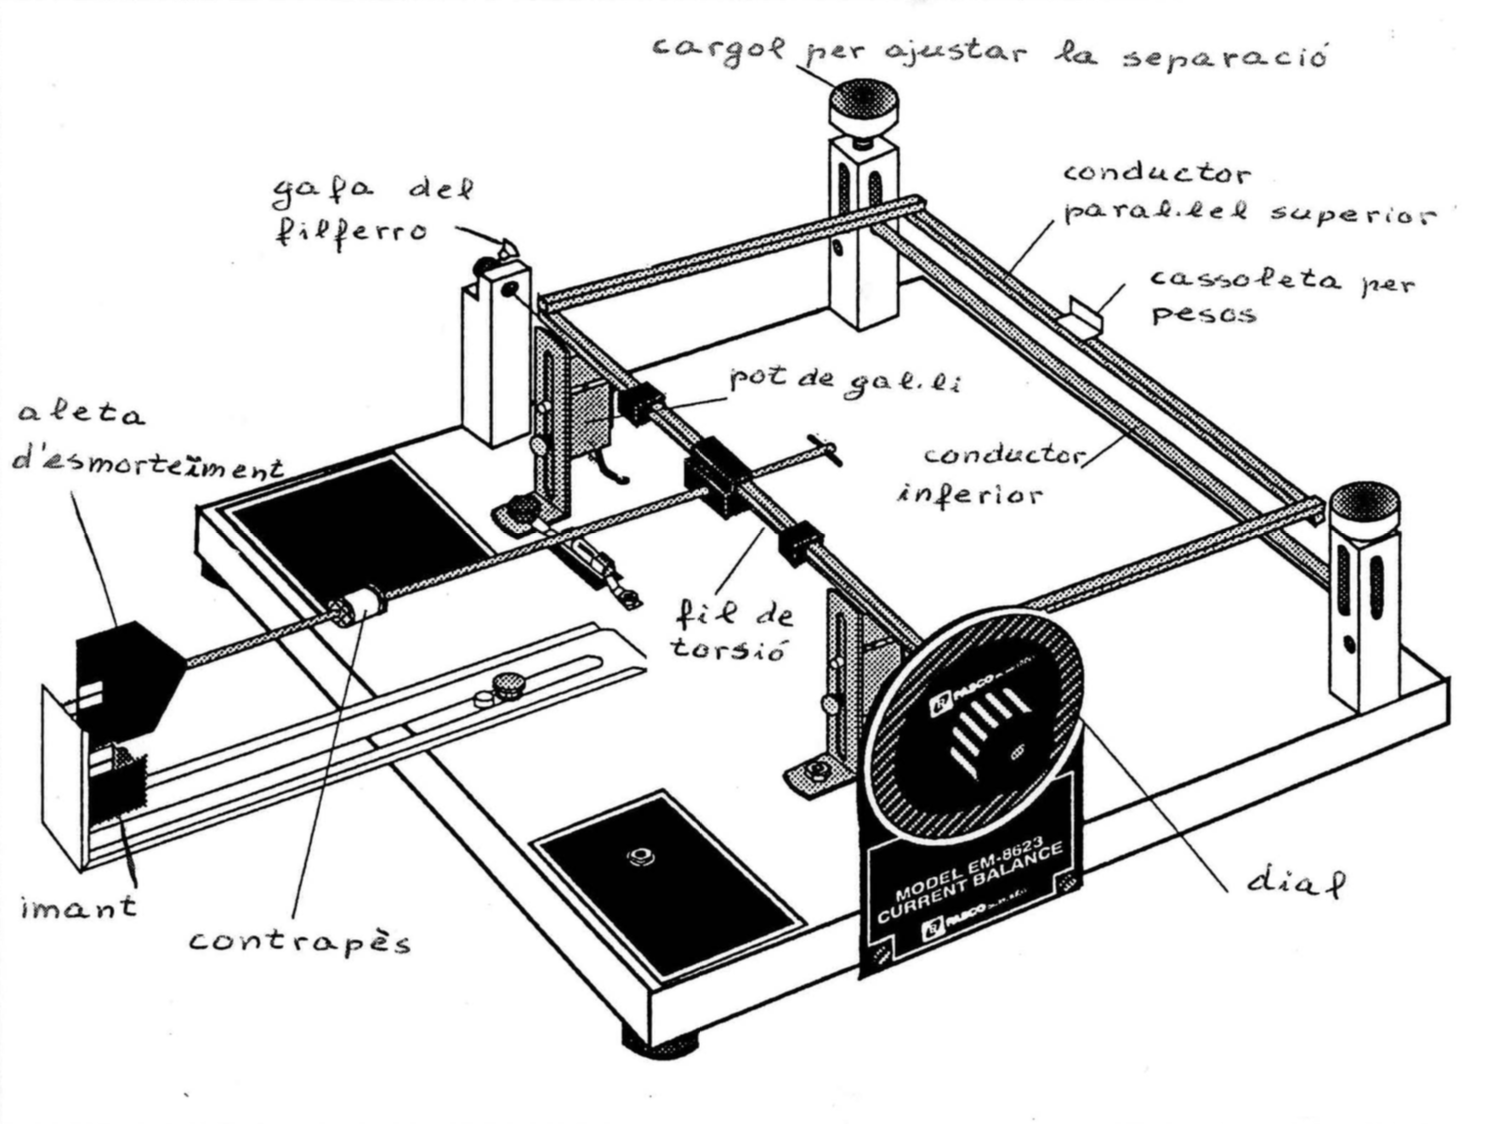
\includegraphics[scale=0.4]{balanca.png}
		\caption{Esquema de la balança de corrents amb els principals elements}
		\label{fig:balanca}
	\end{figure*}

	La balança disposa de dos maneres de determinar la força entre els corrents. Per una banda, disposa d'una cassoleta de pesos on col·locar diferents masses. Sabent que, en el moment que la balança es troba equilibrada, la força gravitatòria sobre la massa és igual a la força entre els corrents es pot determinar aquesta última. Per l'altra banda, la balança també disposa d'un dial i un fil de torsió que poden contrarrestar la força entre els corrents. Sabent que la relació entre els graus que rota el dial i la força que fa és lineal, i coneixent la constant de proporcionalitat es pot determinar també la força entre els corrents.

	Creiem necessari comentar que els corrents s'han disposat en direcció nord-sud terrestre per tal que el camp magnètic de la Terra no influís en els nostres resultats.

	Cal també comentar que el valor que s'ha pres com a acceleració de la gravetat és \SI{9.80665}{m.s^{-2}} sense incertesa, ja que s'ha considerat que és menyspreable enfront a la resta d'incerteses que puguem tenir. S'han pres també sense incertesa els valors de les masses proporcionades al laboratori.

	\subsection{Força vs. Intensitat}
	Per aquesta part de la pràctica s'ha mesurat la intensitat necessària per compensar la força gravitatòria exercida sobre el cable superior per masses de \SIlist{5; 10; 15; 20; 25}{mg}. Posteriorment s'ha aplicat una regressió lineal entre la força i el quadrat de la intensitat per comprovar-ne la correlació predita per l'\cref{eq:forca i corrent}.

	\subsection{Força vs. Distància}
	En aquesta part, s'ha fixat una intensitat i s'ha anat variant la distància entre els cables amb els cargols disposats amb aquest fi. Per cada distància desitjada s'ha determinat la força entre els corrents a partir del dial i el fil de torsió. A les dades preses se'ls hi ha aplicat una regressió lineal entre la força i l'invers de la distància de separació per comprovar la correlació predita per l'\cref{eq:forca i corrent}. A partir del pendent obtingut en la regressió i l'\cref{eq:forca i corrent} s'ha determinat experimentalment la constant $\mu_0$.

	\subsection{Camp Magnètic Terrestre}
	Per aquesta part de l'experiència %Arnau I lof u
	s'han orientat els corrents en direcció est-oest per tal que influís la component radial del camp magnètic terrestre. Per la disposició de la balança i el fet que la força que un camp magnètic exerceix sobre un corrent és perpendicular al pla que defineixen no es pot determinar la component horitzontal del camp magnètic terrestre.

	Posteriorment, s'ha fet circular una intensitat fixa només pel fil superior i s'ha determinat la força que patia a través del dial i el fil de torsió. El camp magnètic s'ha determinat a partir de l'\cref{eq:forca magnetica}. 
	\section{Resultats}
	\subsection{Força vs. Intensitat}
	La \cref{tab:forca v intensitat} mostra les mitjanes de les intensitats necessàries per contrarrestar la força gravitatòria de les diferents masses usades. La \cref{tab:forca v intensitat (detall)}	de l'annex mostra totes les dades per a cada massa. 

	\begin{table*}[h]
		\sffamily \small
		\centering
		\caption{Intensitat mitjana necessària per contrarrestar la força gravitatòria de cada massa.}
		\label{tab:forca v intensitat}
		\begin{tabular}{SSS}
			\toprule
			{Massa (\si{mg})} & {Intensitat (\si{A})} & {Incertesa en la intensitat (\si{A})} \\
			\midrule
			5 & 2.62 & 0.10 \\
			10 & 3.62 & 0.18 \\
			15 & 4.49 & 0.15 \\
			20 & 5.19 & 0.18 \\
			25 & 5.8 & 0.3 \\
			\bottomrule
		\end{tabular}
	\end{table*}

	Amb els valors presentats a la \cref{tab:forca v intensitat} s'ha fet una regressió lineal entre la força entre corrents i el quadrat de la intensitat. La regressió, amb un coeficient $r^2=0.999$, es presenta a la Figura 2. \todo[inline]{Arreglar referència}

	El valor obtingut del pendent de la recta de regressió es de \( m = \data{7.35}{0.08d-6}{N.A^{-2}} \). A partir d'aquest valor i l'\cref{eq:forca i corrent} s'ha determinat \( \mu_0 = \data{1.25}{0.04d-6}{N.A^{-2}} \) que és compatible amb el valor tabulat.
	\subsection{Força vs. Distància}
	Primerament, a través d'una regressió lineal amb un factor de correlació $r^2=0.985$ s'ha determinat la dependència lineal entre la força exercida pel fil de torsió i la rotació del dial, amb un valor de la constant de proporcionalitat de \( k = \data{3.2}{0.2d-7}{N} \). Les dades de la regressió es poden veure a la \cref{tab:regressio forca-angle} i a la Figura A2.1, ambdues a l'annex. \todo[inline]{Arreglar referència} Així, la força es pot determinar per
	\begin{equation} \label{eq:forca i angle}
		F=k\theta
	\end{equation}

	S'ha fixat una intensitat constant de \( I = \data{5.37}{0.02}{A} \) i s'ha mesurat la rotació necessària del dial per contrarrestrar la força entre corrents. La \cref{tab:forca v desplacament} mostra els resultats. 

	\begin{table*}
		\sffamily \small
		\centering
		\caption{Rotació del dial necessària per contrarrestar la força entre corrents a diferents distàncies. La intensitat, fixa, és de \( I = \data{5.37}{0.02}{A} \).}
		\label{tab:forca v desplacament}

		\begin{tabular}{SS}
			\toprule
			{Separació (\si{m}) (\( {} \pm \SI{0.001}{m} \))} &  {Rotació (\si{\degree}) (\( {} \pm \SI{1}{\degree} \))} \\
			\midrule 
			0.010 & 64  \\ 
			0.009 & 63  \\  
			0.008 & 65 \\  
			0.007 & 87  \\  
			0.006 & 129  \\   
			0.005 & 186  \\   
			\bottomrule
		\end{tabular}
	\end{table*}

	Amb les dades de la \cref{tab:forca v desplacament} s'ha realitzat una regressió lineal entre la força entre corrents, calculada a partir de l'\cref{eq:forca i angle}, i l'invers de la distància. La regressió, amb un coeficient $r^2=0.932$, es pot veure a la  Figura 2. \todo[inline]{Arreglar referència}

	El pendent obtingut a partir de la regressió és \( \data{4.1}{0.6d-6}{} \) $n=(4.1\pm0.6)\cdot10^{-6}$. A partir d'aquest valor i l'\cref{eq:forca magnetica} s'ha determinat experimentalment el valor de la constant \( \mu_0 = \data{3.0}{0.4d-6}{N.A^{-2}} \). El resultat no és consistent amb el valor tabulat, possiblement per interferències amb altres elements, però sí de l'orde del valor acceptat.

	\subsection{Camp Magnètic Terrestre}
	La \cref{tab:camp terrestre} mostra tres mesures d'intensitat i les respectives rotacions del dial per tal de compensar la força que el cable pateix degut a la component radial del camp magnètic terrestre. La força s'obté a partir de l'\cref{eq:forca i angle}, i el camp a partir de l'\cref{eq:forca i corrent}.

	\begin{table*}
		\sffamily \small
		\centering
		\caption{Mesures de la component radial del camp magnètic terrestre}
		\label{tab:camp terrestre}
		\begin{tabular}{SSSS}
			\toprule
			{Intensitat (\si{A}) (\( {} \pm \SI{0.01}{A} \))} & {Rotació (\si{\degree}) (\( {} \pm \SI{0.01}{\degree} \))} & {Camp magnètic (\si{nT})} & {Incertesa (\si{nT})} \\
			\midrule
			6.06 & 8 & 1.4d4 & 0.3d4 \\
			6.13 & 8  & 1.4d4 & 0.3d4 \\
			6.57 & 12 & 2.0d4 & 0.4d4 \\ 
			\bottomrule
		\end{tabular}
	\end{table*}

	D'aquesta manera, obtenim, a partir de la mitjana aritmètica dels valors de la \cref{tab:camp terrestre}, un valor de la component radial del camp magnètic terrestre de \( B = \data{1.59}{0.18d-5}{T}  \). El resultat no és consistent amb el valor tabulat del camp magnètic a Madrid l'any 1975, possiblement per interferències amb altres elements, però sí que n'és de l'ordre.

	\section{Conclusions}
	Concloem, primer de tot, que existeix una relació lineal entre la força exercida entre dos corrents com els descrits i el quadrat de la intensitat que hi circula, així com amb l'invers de la distància a què es troben, tal com prediu la llei de Biot-Savart.

	A més, s'ha pogut determinar experimentalment l'ordre de la constant $\mu_0$ a partir de dues regressions lineals i l'assumpció que la llei de Biot-Savart és vàlida. Les possibles discrepàncies amb el valor real es creuen degudes a possibles interferències amb elements del laboratori o a errors sistemàtics.

	Finalment, s'ha determinat també l'ordre del valor de la component radial del camp magnètic terrestre, que coincideix amb el valor tabulat. La component tangencial no s'ha pogut mesurar degut a la disposició de la balança.
\end{multicols*}


% Informe 7
\chapter{Camps magnètics d'espires i bobines}
\begin{resum}
Aquesta pràctica té com a objectiu principal l'estudi dels camps magnètics creats per diferents configuracions d'espires i bobines. Mitjançant una sonda Hall s'han mesurat els camps creats, al seu centre, per espires de radis diferents, així com per conjunts de una, dues i tres espires. De la mateixa manera s'han realitzat mesures del camp magnètic al llarg de l'eix de bobinas de diversos radis.

Amb les dades experimentals s'ha posat a prova la dependència del camp magnètic d'una espira del seu radi i també del nombre d'espires, tal i com prediu la llei de Biot-Savart. També s'ha pogut trobar un valor per a la permeabilitat magnètica del buit, \( \mu_0 \).
\end{resum}
\todo{error relatiu comès}

\section{Introducció}
En la primera part de la pràctica s'estudiarà el camp magnètic degut a conjunts d'espires. Si considerem un conjunt de \( N \) espires de radi \( R \) per les que hi circula un corrent constant \( I \), un càlcul elemental amb la llei de Biot-Savart ens dóna que el camp magnètic \( \vec{B} \) al seu centre és
\begin{equation}\label{eq:camp espira}
  \vec{B}=\frac{\mu_0 I N}{2 R}\vec{e}_z,
\end{equation}
on \( \vec{e}_z \) és el vector unitari perpendicular al pla de les espires. Així doncs esperem poder observar les relacions \( B \propto R^{-1} \) i \( B \propto N \). 

Pel que fa al camp magnètic d'una bobina, sabem que en el cas d'una bobina infinita el camp en el seu interior és constant i nul a l'exterior. En el cas d'una bobina finita de longitud \( L \), radi \( R \), \( N \) voltes i per la qual hi passa una intensitat constant \( I \), el camp a punts del seu eix es pot trobar de manera exacta mitjançant la llei de Biot-Savart i resulta
\begin{equation}\label{eq:camp bobina}
  \vec{B}=\frac{\mu_0 I N}{2 L}\left(\frac{z + L/2}{\sqrt{R^2+(z+L/2)^2}} - \frac{z - L/2}{\sqrt{R^2 + (z - L/2)^2}}\right) \vec{e}_z,
\end{equation}
on \( z \) és la posició de la sonda al llarg de l'eix de la bobina ---fixant \( z = 0 \) al seu centre--- i \( \vec{e}_z \) és el vector unitari para\l.lel a l'eix. Quan \( L \gg R \) aleshores l'\cref{eq:camp bobina} dóna lloc a un camp que és gairebé constant per \( \abs{z} < L/2 \) i que decau molt depressa cap a 0 quan \( \abs{z} > L/2 \). 

\section{Mètode experimental}
\subsection{Espires}
Per a realitzar les mesures s'ha fet servir la disposició que es mostra a la \cref{fig:circuit teslametre}. Les espires i la sonda estaven cada una sobre un suport de manera que la sonda estigués a la mateixa alçada que el centre de l'espira. La sonda també estava muntada sobre una rail de manera que es mantingués sempre sobre l'eix perpendicular de les espires.

\begin{figure}[htb]
  \centering \small \sffamily
  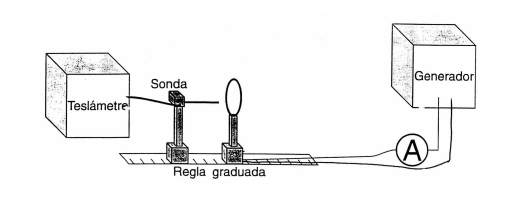
\includegraphics{circuit-teslametre.png}
  \caption{Esquema del circuit emprat per a mesurar el camp magnètic}
  \label{fig:circuit teslametre}
\end{figure}

El corrent subministrat per la font es va fixar a \SI{4.00}{A} i tot seguit la sonda es va desplaçar fins al centre de l'espira ---de la qual ja s'havia mesurat el radi---. Cal mencionar que el sensor de camp magnètic no es troba exactament a la punta de la sonda, de manera que és complicat determinar exactament quan és que efectivament s'estava mesurant el camp al centre. Com que, d'acord amb el resultat teòric, el camp magnètic s'una espira és màxim al seu centre, es va considerar el màxim valor registrat pel teslàmetre. Degut a la seva alta sensibilitat, el teslàmetre trigava un temps considerable a estabilitzar la seva lectura després de canvis bruscos en el camp magnètic. 

S'han pres sis mesures del camp per a cada espira---tres en total, cada una amb un radi diferent. Tres amb un sentit del corrent i tres amb el corrent en sentit oposat. Aleshores s'ha fet el promig de les sis lectures per a minimitzar errors aleatoris deguts a fluctuacions en la mesura del teslàmetre.   

Posteriorment s'ha mesurat el camp al centre del conjunt de 1, 2 i 3 espires seguint el mateix procediment.

\subsection{Bobines}
Per la mesura del camp a l'interior de les bobines s'ha fet servir el mateix circuit que es mostra a la \cref{fig:circuit teslametre}.

Ajustant la intensitat a \data{1.00}{0.01}{A} a l'amperímetre, s'ha mesurat el camp a diversos punts a l'interior de la bobina. Per fer-ho s'ha ajustat l'alçada de la sonda de manera que aquesta quedi sobre l'eix de la bobina. Començant pel punt immediatament a l'exterior de la bobina s'ha fet avançar la sonda sobre el regle mesurant el camp cada \SI{3}{cm} de manera que n'han resultat 8 mesures a diferents punts de l'eix.

Aquest mateix procediment s'ha repetit per cada una de les bobines diferents.  

\section{Resultats}
\subsection{Espires}\label{sec:espires}
Com s'ha mencionat anteriorment, en aquesta secció es presenten els resultats relatius a la part de la pràctica referent a les espires. A la \cref{tab:camp espires en funcio de r} es presenten les mesures del camp magnètic al centre d'una espira en funció del seu radi. 

\begin{table}[htb]
  \centering \small \sffamily
  \caption{Taula de valors teòrics i experimentals}
  \label{tab:camp espires en funcio de r}
	\begin{tabular}{SSS}
		\toprule
		{Radi (\data{}{0.2}{cm})} & { \( B_{\textsf{exp}}\ (\SI{d-5}{T}) \) } & { \( B_{\textsf{teò}}\ (\SI{d-5}{T}) \) } \\
		\midrule
		3.0 & 7.3\pm1.4 & 8.4\pm0.4 \\
		4.3 & 6.0\pm1.6 & 5.9\pm0.2 \\
		6.0 & 5.0\pm1.6 & 4.2\pm0.1 \\
		\bottomrule
	\end{tabular}
\end{table}

Les incerteses dels camps experimentals de la \cref{tab:camp espires en funcio de r} han estat calculades segons la desviació estàndard de les diferents mesures realitzades. Pel que fa a les incerteses teòriques, aquestes han estat calculades per propagació d'incerteses de la fórmula \cref{eq:camp espira}. Com podem veure en els tres casos, els valors experimentals amb els seus respectius intervals d'incertesa coincideixen en alguns punts amb els valors teòrics i els seus intervals, per tant els resultats són compatibles. Es pot observar que l'incertesa dels resultats experimentals és considerablement major. Això és degut a les imprecisions dels aparells emprats per a la mesura dels camps, especialment a les contínues fluctuacions del teslàmetre. 

Tanmateix, el fet més rellevant que podem observar és la disminució del camp a l'interior de l'espira a mesura que augmenta el seu radi. Aquest resultat ja era el que esperavem teòricament. Per fer més èmfasi en aquest fet es presenta la gràfica de lacref{fig:camp espira}, on es representa el camp magnètic al centre en funció del radi de l'espira.
\begin{figure}[htb]
  \centering
  % 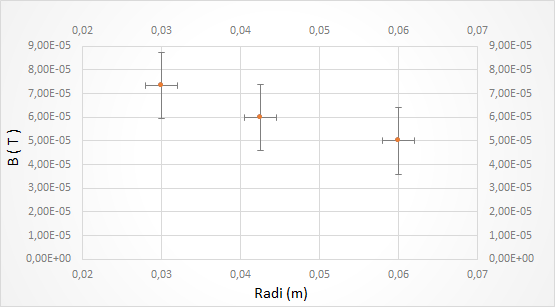
\includegraphics[width=100mm]{graf1.png}
  \caption{Camp magnètic al centre en funció del radi de l'espira}
  \label{fig:camp espira}
\end{figure}

Com es comentava, s'observa que el camp a l'interior es va  atenuant a mesura que s'augmenta el radi de l'espira. Tot i que és difícil d'apreciar ja que només s'ha fet la mesura amb tres radis diferents, es pot comprovar numèricament que el camp magnètic decau com \( \frac{1}{R} \). Aquesta és per tant la forma de funció que observaríem si es tinguessin valors infinits de radis d'espires i els seus camps respectius.

La taula \cref{tab:camp espires en funcio de n} presenta els camp magnètics teòrics i experimentals al centre dels conjunts de 1, 2 i 3 espires. 

\begin{table}[htb]
	\centering \small \sffamily
	\caption{Valors teòrics i experimentals del camp magnètic al centre d'un conjunt de \( N \) espires}
	\label{tab:camp espires en funcio de n}
	\begin{tabular}{SSS}
		\toprule
		{Nombre d'espires \( N \)} & { \( B_{\textsf{exp}}\ (\SI{d-5}{T}) \) } & { \( B_{\textsf{teò}}\ (\SI{d-5}{T}) \) } \\
		\midrule
		1 & 5.0\pm1.6 & 4.2\pm0.1 \\
		2 & 8.8\pm1.5 & 8.4\pm0.2 \\
		3 & 12.3\pm1.5 & 12.6\pm0.3 \\
		\bottomrule
	\end{tabular}
\end{table}

Podem observar que en aquest cas els intervals dels camps teòrics i experimentals també se solapen i per tant les observacions satisfan l'esperat. Altra vegada tornem a tenir incerteses majors pels valors experimentals pel mateix fet anteriorment mencionat. Els resultats ens permeten observar que com més espires introduïm al conjunt més intens es torna el camp al centre d'aquest. Aquesta dependència es pot observar clarament al gràfic experimental del camp al centre en funció del nombre d'espires que s'exposa a la \cref{fig:camp vs n}.

\begin{figure}[htb]
  \centering
  % 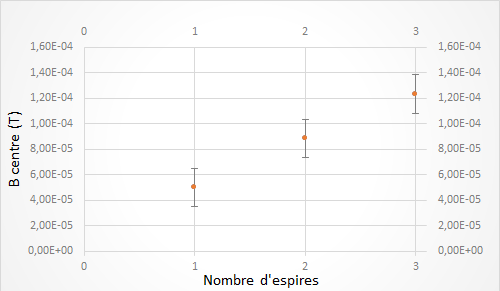
\includegraphics[width=100mm]{graf2.png}
  \caption{Camp al centre en funció del nombre d'espires}
  \label{fig:camp vs n}
\end{figure}

Podem veure a la regressió de la \cref{fig:camp vs n} que aquesta dependència és lineal com s'esperava dels valors teòrics obtinguts a partir de la \cref{eq:camp espira}. El valor de $\mu_{0}$ obtingut a partir de la regressió tenint en compte que el pendent segons \cref{eq:camp espira} és $\frac{\mu_{0}I}{2R}$  s'obté un valor de $\mu_{0} = \data{1.10}{0.37d-6}{N.A^{-2}} $ que és compatible amb el valor teòric de $\mu_{0}\approx \SI{1.26d-6}{N.A^{-2}} $. Així doncs, vist que el camp augmenta de manera directament proporcional al nombre d'espires, els resultats d'aquest apartat queden interpretats.

\subsection{Bobines}\label{sec:bobines}
\begin{figure}[tp]
	\sffamily \small
	\centering
	% GNUPLOT: LaTeX picture with Postscript
\begingroup
\sffamily \small
  \makeatletter
  \providecommand\color[2][]{%
    \GenericError{(gnuplot) \space\space\space\@spaces}{%
      Package color not loaded in conjunction with
      terminal option `colourtext'%
    }{See the gnuplot documentation for explanation.%
    }{Either use 'blacktext' in gnuplot or load the package
      color.sty in LaTeX.}%
    \renewcommand\color[2][]{}%
  }%
  \providecommand\includegraphics[2][]{%
    \GenericError{(gnuplot) \space\space\space\@spaces}{%
      Package graphicx or graphics not loaded%
    }{See the gnuplot documentation for explanation.%
    }{The gnuplot epslatex terminal needs graphicx.sty or graphics.sty.}%
    \renewcommand\includegraphics[2][]{}%
  }%
  \providecommand\rotatebox[2]{#2}%
  \@ifundefined{ifGPcolor}{%
    \newif\ifGPcolor
    \GPcolortrue
  }{}%
  \@ifundefined{ifGPblacktext}{%
    \newif\ifGPblacktext
    \GPblacktextfalse
  }{}%
  % define a \g@addto@macro without @ in the name:
  \let\gplgaddtomacro\g@addto@macro
  % define empty templates for all commands taking text:
  \gdef\gplbacktext{}%
  \gdef\gplfronttext{}%
  \makeatother
  \ifGPblacktext
    % no textcolor at all
    \def\colorrgb#1{}%
    \def\colorgray#1{}%
  \else
    % gray or color?
    \ifGPcolor
      \def\colorrgb#1{\color[rgb]{#1}}%
      \def\colorgray#1{\color[gray]{#1}}%
      \expandafter\def\csname LTw\endcsname{\color{white}}%
      \expandafter\def\csname LTb\endcsname{\color{black}}%
      \expandafter\def\csname LTa\endcsname{\color{black}}%
      \expandafter\def\csname LT0\endcsname{\color[rgb]{1,0,0}}%
      \expandafter\def\csname LT1\endcsname{\color[rgb]{0,1,0}}%
      \expandafter\def\csname LT2\endcsname{\color[rgb]{0,0,1}}%
      \expandafter\def\csname LT3\endcsname{\color[rgb]{1,0,1}}%
      \expandafter\def\csname LT4\endcsname{\color[rgb]{0,1,1}}%
      \expandafter\def\csname LT5\endcsname{\color[rgb]{1,1,0}}%
      \expandafter\def\csname LT6\endcsname{\color[rgb]{0,0,0}}%
      \expandafter\def\csname LT7\endcsname{\color[rgb]{1,0.3,0}}%
      \expandafter\def\csname LT8\endcsname{\color[rgb]{0.5,0.5,0.5}}%
    \else
      % gray
      \def\colorrgb#1{\color{black}}%
      \def\colorgray#1{\color[gray]{#1}}%
      \expandafter\def\csname LTw\endcsname{\color{white}}%
      \expandafter\def\csname LTb\endcsname{\color{black}}%
      \expandafter\def\csname LTa\endcsname{\color{black}}%
      \expandafter\def\csname LT0\endcsname{\color{black}}%
      \expandafter\def\csname LT1\endcsname{\color{black}}%
      \expandafter\def\csname LT2\endcsname{\color{black}}%
      \expandafter\def\csname LT3\endcsname{\color{black}}%
      \expandafter\def\csname LT4\endcsname{\color{black}}%
      \expandafter\def\csname LT5\endcsname{\color{black}}%
      \expandafter\def\csname LT6\endcsname{\color{black}}%
      \expandafter\def\csname LT7\endcsname{\color{black}}%
      \expandafter\def\csname LT8\endcsname{\color{black}}%
    \fi
  \fi
    \setlength{\unitlength}{0.0500bp}%
    \ifx\gptboxheight\undefined%
      \newlength{\gptboxheight}%
      \newlength{\gptboxwidth}%
      \newsavebox{\gptboxtext}%
    \fi%
    \setlength{\fboxrule}{0.5pt}%
    \setlength{\fboxsep}{1pt}%
\begin{picture}(5668.00,3400.00)%
    \gplgaddtomacro\gplbacktext{%
      \csname LTb\endcsname%%
      \put(946,704){\makebox(0,0)[r]{\strut{}\num{0}}}%
      \put(946,1117){\makebox(0,0)[r]{\strut{}\num{0.5}}}%
      \put(946,1529){\makebox(0,0)[r]{\strut{}\num{1}}}%
      \put(946,1942){\makebox(0,0)[r]{\strut{}\num{1.5}}}%
      \put(946,2354){\makebox(0,0)[r]{\strut{}\num{2}}}%
      \put(946,2767){\makebox(0,0)[r]{\strut{}\num{2.5}}}%
      \put(946,3179){\makebox(0,0)[r]{\strut{}\num{3}}}%
      \put(1078,484){\makebox(0,0){\strut{}\num{-15}}}%
      \put(1777,484){\makebox(0,0){\strut{}\num{-10}}}%
      \put(2476,484){\makebox(0,0){\strut{}\num{-5}}}%
      \put(3175,484){\makebox(0,0){\strut{}\num{0}}}%
      \put(3873,484){\makebox(0,0){\strut{}\num{5}}}%
      \put(4572,484){\makebox(0,0){\strut{}\num{10}}}%
      \put(5271,484){\makebox(0,0){\strut{}\num{15}}}%
    }%
    \gplgaddtomacro\gplfronttext{%
      \csname LTb\endcsname%%
      \put(198,1941){\rotatebox{-270}{\makebox(0,0){\strut{}$\mathsf{B \ (\si{mT})}$}}}%
      \put(3174,154){\makebox(0,0){\strut{}$\mathsf{z \ (\si{cm})}$}}%
    }%
    \gplbacktext
    \put(0,0){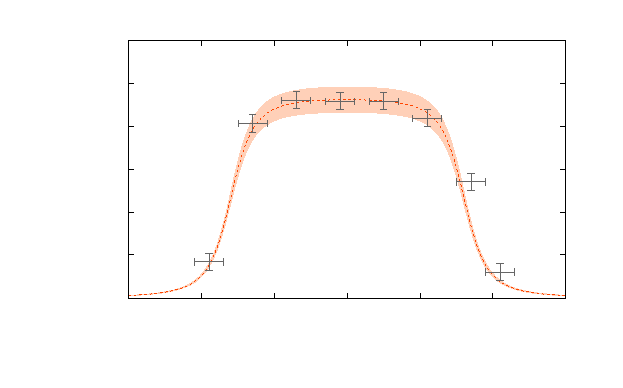
\includegraphics{camp-300-33}}%
    \gplfronttext
  \end{picture}%
\endgroup

	\caption{Camp magnètic al llarg de l'eix d'una bobina de 300 voltes, longitud \SI{16}{cm} i diàmetre \SI{3.3}{cm} per la que hi passa un corrent constant de \SI{1}{A}.}
	\label{fig:camp 300/33}
\end{figure}

\begin{figure}[tp]
	\sffamily \small
	\centering
	% GNUPLOT: LaTeX picture with Postscript
\begingroup
\sffamily \small
  \makeatletter
  \providecommand\color[2][]{%
    \GenericError{(gnuplot) \space\space\space\@spaces}{%
      Package color not loaded in conjunction with
      terminal option `colourtext'%
    }{See the gnuplot documentation for explanation.%
    }{Either use 'blacktext' in gnuplot or load the package
      color.sty in LaTeX.}%
    \renewcommand\color[2][]{}%
  }%
  \providecommand\includegraphics[2][]{%
    \GenericError{(gnuplot) \space\space\space\@spaces}{%
      Package graphicx or graphics not loaded%
    }{See the gnuplot documentation for explanation.%
    }{The gnuplot epslatex terminal needs graphicx.sty or graphics.sty.}%
    \renewcommand\includegraphics[2][]{}%
  }%
  \providecommand\rotatebox[2]{#2}%
  \@ifundefined{ifGPcolor}{%
    \newif\ifGPcolor
    \GPcolortrue
  }{}%
  \@ifundefined{ifGPblacktext}{%
    \newif\ifGPblacktext
    \GPblacktextfalse
  }{}%
  % define a \g@addto@macro without @ in the name:
  \let\gplgaddtomacro\g@addto@macro
  % define empty templates for all commands taking text:
  \gdef\gplbacktext{}%
  \gdef\gplfronttext{}%
  \makeatother
  \ifGPblacktext
    % no textcolor at all
    \def\colorrgb#1{}%
    \def\colorgray#1{}%
  \else
    % gray or color?
    \ifGPcolor
      \def\colorrgb#1{\color[rgb]{#1}}%
      \def\colorgray#1{\color[gray]{#1}}%
      \expandafter\def\csname LTw\endcsname{\color{white}}%
      \expandafter\def\csname LTb\endcsname{\color{black}}%
      \expandafter\def\csname LTa\endcsname{\color{black}}%
      \expandafter\def\csname LT0\endcsname{\color[rgb]{1,0,0}}%
      \expandafter\def\csname LT1\endcsname{\color[rgb]{0,1,0}}%
      \expandafter\def\csname LT2\endcsname{\color[rgb]{0,0,1}}%
      \expandafter\def\csname LT3\endcsname{\color[rgb]{1,0,1}}%
      \expandafter\def\csname LT4\endcsname{\color[rgb]{0,1,1}}%
      \expandafter\def\csname LT5\endcsname{\color[rgb]{1,1,0}}%
      \expandafter\def\csname LT6\endcsname{\color[rgb]{0,0,0}}%
      \expandafter\def\csname LT7\endcsname{\color[rgb]{1,0.3,0}}%
      \expandafter\def\csname LT8\endcsname{\color[rgb]{0.5,0.5,0.5}}%
    \else
      % gray
      \def\colorrgb#1{\color{black}}%
      \def\colorgray#1{\color[gray]{#1}}%
      \expandafter\def\csname LTw\endcsname{\color{white}}%
      \expandafter\def\csname LTb\endcsname{\color{black}}%
      \expandafter\def\csname LTa\endcsname{\color{black}}%
      \expandafter\def\csname LT0\endcsname{\color{black}}%
      \expandafter\def\csname LT1\endcsname{\color{black}}%
      \expandafter\def\csname LT2\endcsname{\color{black}}%
      \expandafter\def\csname LT3\endcsname{\color{black}}%
      \expandafter\def\csname LT4\endcsname{\color{black}}%
      \expandafter\def\csname LT5\endcsname{\color{black}}%
      \expandafter\def\csname LT6\endcsname{\color{black}}%
      \expandafter\def\csname LT7\endcsname{\color{black}}%
      \expandafter\def\csname LT8\endcsname{\color{black}}%
    \fi
  \fi
    \setlength{\unitlength}{0.0500bp}%
    \ifx\gptboxheight\undefined%
      \newlength{\gptboxheight}%
      \newlength{\gptboxwidth}%
      \newsavebox{\gptboxtext}%
    \fi%
    \setlength{\fboxrule}{0.5pt}%
    \setlength{\fboxsep}{1pt}%
\begin{picture}(5668.00,3400.00)%
    \gplgaddtomacro\gplbacktext{%
      \csname LTb\endcsname%%
      \put(946,704){\makebox(0,0)[r]{\strut{}\num{0}}}%
      \put(946,1199){\makebox(0,0)[r]{\strut{}\num{0.2}}}%
      \put(946,1694){\makebox(0,0)[r]{\strut{}\num{0.4}}}%
      \put(946,2189){\makebox(0,0)[r]{\strut{}\num{0.6}}}%
      \put(946,2684){\makebox(0,0)[r]{\strut{}\num{0.8}}}%
      \put(946,3179){\makebox(0,0)[r]{\strut{}\num{1}}}%
      \put(1078,484){\makebox(0,0){\strut{}\num{-15}}}%
      \put(1777,484){\makebox(0,0){\strut{}\num{-10}}}%
      \put(2476,484){\makebox(0,0){\strut{}\num{-5}}}%
      \put(3175,484){\makebox(0,0){\strut{}\num{0}}}%
      \put(3873,484){\makebox(0,0){\strut{}\num{5}}}%
      \put(4572,484){\makebox(0,0){\strut{}\num{10}}}%
      \put(5271,484){\makebox(0,0){\strut{}\num{15}}}%
    }%
    \gplgaddtomacro\gplfronttext{%
      \csname LTb\endcsname%%
      \put(198,1941){\rotatebox{-270}{\makebox(0,0){\strut{}$\mathsf{B \ (\si{mT})}$}}}%
      \put(3174,154){\makebox(0,0){\strut{}$\mathsf{z \ (\si{cm})}$}}%
    }%
    \gplbacktext
    \put(0,0){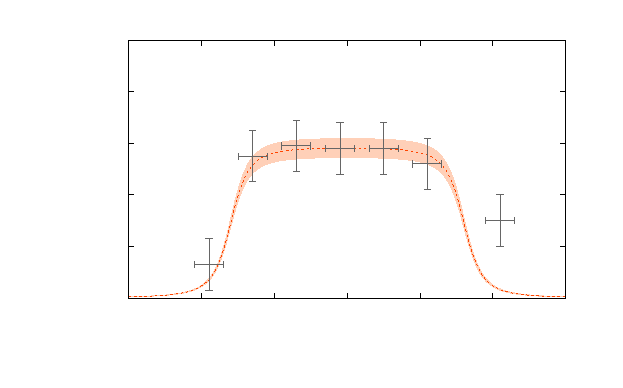
\includegraphics{camp-75-26}}%
    \gplfronttext
  \end{picture}%
\endgroup

	\caption{Camp magnètic al llarg de l'eix d'una bobina de 75 voltes, longitud \SI{16}{cm} i diàmetre \SI{2.6}{cm} per la que hi passa un corrent constant de \SI{1}{A}.}
	\label{fig:camp 75/26}
\end{figure}

\begin{figure}[tp]
	\sffamily \small
	\centering
	% GNUPLOT: LaTeX picture with Postscript
\begingroup
\sffamily \small
  \makeatletter
  \providecommand\color[2][]{%
    \GenericError{(gnuplot) \space\space\space\@spaces}{%
      Package color not loaded in conjunction with
      terminal option `colourtext'%
    }{See the gnuplot documentation for explanation.%
    }{Either use 'blacktext' in gnuplot or load the package
      color.sty in LaTeX.}%
    \renewcommand\color[2][]{}%
  }%
  \providecommand\includegraphics[2][]{%
    \GenericError{(gnuplot) \space\space\space\@spaces}{%
      Package graphicx or graphics not loaded%
    }{See the gnuplot documentation for explanation.%
    }{The gnuplot epslatex terminal needs graphicx.sty or graphics.sty.}%
    \renewcommand\includegraphics[2][]{}%
  }%
  \providecommand\rotatebox[2]{#2}%
  \@ifundefined{ifGPcolor}{%
    \newif\ifGPcolor
    \GPcolortrue
  }{}%
  \@ifundefined{ifGPblacktext}{%
    \newif\ifGPblacktext
    \GPblacktextfalse
  }{}%
  % define a \g@addto@macro without @ in the name:
  \let\gplgaddtomacro\g@addto@macro
  % define empty templates for all commands taking text:
  \gdef\gplbacktext{}%
  \gdef\gplfronttext{}%
  \makeatother
  \ifGPblacktext
    % no textcolor at all
    \def\colorrgb#1{}%
    \def\colorgray#1{}%
  \else
    % gray or color?
    \ifGPcolor
      \def\colorrgb#1{\color[rgb]{#1}}%
      \def\colorgray#1{\color[gray]{#1}}%
      \expandafter\def\csname LTw\endcsname{\color{white}}%
      \expandafter\def\csname LTb\endcsname{\color{black}}%
      \expandafter\def\csname LTa\endcsname{\color{black}}%
      \expandafter\def\csname LT0\endcsname{\color[rgb]{1,0,0}}%
      \expandafter\def\csname LT1\endcsname{\color[rgb]{0,1,0}}%
      \expandafter\def\csname LT2\endcsname{\color[rgb]{0,0,1}}%
      \expandafter\def\csname LT3\endcsname{\color[rgb]{1,0,1}}%
      \expandafter\def\csname LT4\endcsname{\color[rgb]{0,1,1}}%
      \expandafter\def\csname LT5\endcsname{\color[rgb]{1,1,0}}%
      \expandafter\def\csname LT6\endcsname{\color[rgb]{0,0,0}}%
      \expandafter\def\csname LT7\endcsname{\color[rgb]{1,0.3,0}}%
      \expandafter\def\csname LT8\endcsname{\color[rgb]{0.5,0.5,0.5}}%
    \else
      % gray
      \def\colorrgb#1{\color{black}}%
      \def\colorgray#1{\color[gray]{#1}}%
      \expandafter\def\csname LTw\endcsname{\color{white}}%
      \expandafter\def\csname LTb\endcsname{\color{black}}%
      \expandafter\def\csname LTa\endcsname{\color{black}}%
      \expandafter\def\csname LT0\endcsname{\color{black}}%
      \expandafter\def\csname LT1\endcsname{\color{black}}%
      \expandafter\def\csname LT2\endcsname{\color{black}}%
      \expandafter\def\csname LT3\endcsname{\color{black}}%
      \expandafter\def\csname LT4\endcsname{\color{black}}%
      \expandafter\def\csname LT5\endcsname{\color{black}}%
      \expandafter\def\csname LT6\endcsname{\color{black}}%
      \expandafter\def\csname LT7\endcsname{\color{black}}%
      \expandafter\def\csname LT8\endcsname{\color{black}}%
    \fi
  \fi
    \setlength{\unitlength}{0.0500bp}%
    \ifx\gptboxheight\undefined%
      \newlength{\gptboxheight}%
      \newlength{\gptboxwidth}%
      \newsavebox{\gptboxtext}%
    \fi%
    \setlength{\fboxrule}{0.5pt}%
    \setlength{\fboxsep}{1pt}%
\begin{picture}(5668.00,3400.00)%
    \gplgaddtomacro\gplbacktext{%
      \csname LTb\endcsname%%
      \put(946,704){\makebox(0,0)[r]{\strut{}\num{0}}}%
      \put(946,1323){\makebox(0,0)[r]{\strut{}\num{0.5}}}%
      \put(946,1942){\makebox(0,0)[r]{\strut{}\num{1}}}%
      \put(946,2560){\makebox(0,0)[r]{\strut{}\num{1.5}}}%
      \put(946,3179){\makebox(0,0)[r]{\strut{}\num{2}}}%
      \put(1078,484){\makebox(0,0){\strut{}\num{-15}}}%
      \put(1777,484){\makebox(0,0){\strut{}\num{-10}}}%
      \put(2476,484){\makebox(0,0){\strut{}\num{-5}}}%
      \put(3175,484){\makebox(0,0){\strut{}\num{0}}}%
      \put(3873,484){\makebox(0,0){\strut{}\num{5}}}%
      \put(4572,484){\makebox(0,0){\strut{}\num{10}}}%
      \put(5271,484){\makebox(0,0){\strut{}\num{15}}}%
    }%
    \gplgaddtomacro\gplfronttext{%
      \csname LTb\endcsname%%
      \put(198,1941){\rotatebox{-270}{\makebox(0,0){\strut{}$\mathsf{B \ (\si{mT})}$}}}%
      \put(3174,154){\makebox(0,0){\strut{}$\mathsf{z \ (\si{cm})}$}}%
    }%
    \gplbacktext
    \put(0,0){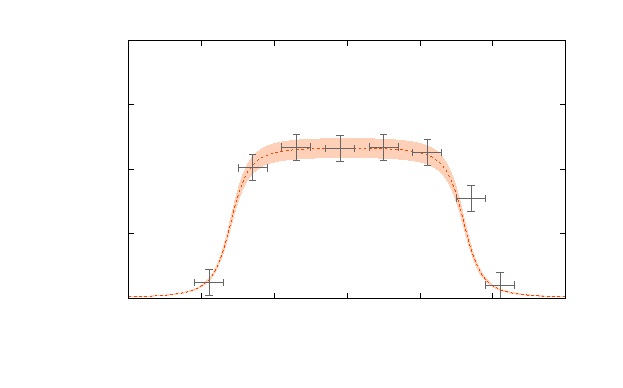
\includegraphics{camp-150-26}}%
    \gplfronttext
  \end{picture}%
\endgroup

	\caption{Camp magnètic al llarg de l'eix d'una bobina de 150 voltes, longitud \SI{16}{cm} i diàmetre \SI{2.6}{cm} per la que hi passa un corrent constant de \SI{1}{A}.}
	\label{fig:camp 150/26}
\end{figure}

\begin{figure}[tp]
	\sffamily \small
	\centering
	% GNUPLOT: LaTeX picture with Postscript
\begingroup
\sffamily \small
  \makeatletter
  \providecommand\color[2][]{%
    \GenericError{(gnuplot) \space\space\space\@spaces}{%
      Package color not loaded in conjunction with
      terminal option `colourtext'%
    }{See the gnuplot documentation for explanation.%
    }{Either use 'blacktext' in gnuplot or load the package
      color.sty in LaTeX.}%
    \renewcommand\color[2][]{}%
  }%
  \providecommand\includegraphics[2][]{%
    \GenericError{(gnuplot) \space\space\space\@spaces}{%
      Package graphicx or graphics not loaded%
    }{See the gnuplot documentation for explanation.%
    }{The gnuplot epslatex terminal needs graphicx.sty or graphics.sty.}%
    \renewcommand\includegraphics[2][]{}%
  }%
  \providecommand\rotatebox[2]{#2}%
  \@ifundefined{ifGPcolor}{%
    \newif\ifGPcolor
    \GPcolortrue
  }{}%
  \@ifundefined{ifGPblacktext}{%
    \newif\ifGPblacktext
    \GPblacktextfalse
  }{}%
  % define a \g@addto@macro without @ in the name:
  \let\gplgaddtomacro\g@addto@macro
  % define empty templates for all commands taking text:
  \gdef\gplbacktext{}%
  \gdef\gplfronttext{}%
  \makeatother
  \ifGPblacktext
    % no textcolor at all
    \def\colorrgb#1{}%
    \def\colorgray#1{}%
  \else
    % gray or color?
    \ifGPcolor
      \def\colorrgb#1{\color[rgb]{#1}}%
      \def\colorgray#1{\color[gray]{#1}}%
      \expandafter\def\csname LTw\endcsname{\color{white}}%
      \expandafter\def\csname LTb\endcsname{\color{black}}%
      \expandafter\def\csname LTa\endcsname{\color{black}}%
      \expandafter\def\csname LT0\endcsname{\color[rgb]{1,0,0}}%
      \expandafter\def\csname LT1\endcsname{\color[rgb]{0,1,0}}%
      \expandafter\def\csname LT2\endcsname{\color[rgb]{0,0,1}}%
      \expandafter\def\csname LT3\endcsname{\color[rgb]{1,0,1}}%
      \expandafter\def\csname LT4\endcsname{\color[rgb]{0,1,1}}%
      \expandafter\def\csname LT5\endcsname{\color[rgb]{1,1,0}}%
      \expandafter\def\csname LT6\endcsname{\color[rgb]{0,0,0}}%
      \expandafter\def\csname LT7\endcsname{\color[rgb]{1,0.3,0}}%
      \expandafter\def\csname LT8\endcsname{\color[rgb]{0.5,0.5,0.5}}%
    \else
      % gray
      \def\colorrgb#1{\color{black}}%
      \def\colorgray#1{\color[gray]{#1}}%
      \expandafter\def\csname LTw\endcsname{\color{white}}%
      \expandafter\def\csname LTb\endcsname{\color{black}}%
      \expandafter\def\csname LTa\endcsname{\color{black}}%
      \expandafter\def\csname LT0\endcsname{\color{black}}%
      \expandafter\def\csname LT1\endcsname{\color{black}}%
      \expandafter\def\csname LT2\endcsname{\color{black}}%
      \expandafter\def\csname LT3\endcsname{\color{black}}%
      \expandafter\def\csname LT4\endcsname{\color{black}}%
      \expandafter\def\csname LT5\endcsname{\color{black}}%
      \expandafter\def\csname LT6\endcsname{\color{black}}%
      \expandafter\def\csname LT7\endcsname{\color{black}}%
      \expandafter\def\csname LT8\endcsname{\color{black}}%
    \fi
  \fi
    \setlength{\unitlength}{0.0500bp}%
    \ifx\gptboxheight\undefined%
      \newlength{\gptboxheight}%
      \newlength{\gptboxwidth}%
      \newsavebox{\gptboxtext}%
    \fi%
    \setlength{\fboxrule}{0.5pt}%
    \setlength{\fboxsep}{1pt}%
\begin{picture}(5668.00,3400.00)%
    \gplgaddtomacro\gplbacktext{%
      \csname LTb\endcsname%%
      \put(946,704){\makebox(0,0)[r]{\strut{}\num{0}}}%
      \put(946,1013){\makebox(0,0)[r]{\strut{}\num{0.5}}}%
      \put(946,1323){\makebox(0,0)[r]{\strut{}\num{1}}}%
      \put(946,1632){\makebox(0,0)[r]{\strut{}\num{1.5}}}%
      \put(946,1942){\makebox(0,0)[r]{\strut{}\num{2}}}%
      \put(946,2251){\makebox(0,0)[r]{\strut{}\num{2.5}}}%
      \put(946,2560){\makebox(0,0)[r]{\strut{}\num{3}}}%
      \put(946,2870){\makebox(0,0)[r]{\strut{}\num{3.5}}}%
      \put(946,3179){\makebox(0,0)[r]{\strut{}\num{4}}}%
      \put(1078,484){\makebox(0,0){\strut{}\num{-15}}}%
      \put(1777,484){\makebox(0,0){\strut{}\num{-10}}}%
      \put(2476,484){\makebox(0,0){\strut{}\num{-5}}}%
      \put(3175,484){\makebox(0,0){\strut{}\num{0}}}%
      \put(3873,484){\makebox(0,0){\strut{}\num{5}}}%
      \put(4572,484){\makebox(0,0){\strut{}\num{10}}}%
      \put(5271,484){\makebox(0,0){\strut{}\num{15}}}%
    }%
    \gplgaddtomacro\gplfronttext{%
      \csname LTb\endcsname%%
      \put(198,1941){\rotatebox{-270}{\makebox(0,0){\strut{}$\mathsf{B \ (\si{mT})}$}}}%
      \put(3174,154){\makebox(0,0){\strut{}$\mathsf{z \ (\si{cm})}$}}%
    }%
    \gplbacktext
    \put(0,0){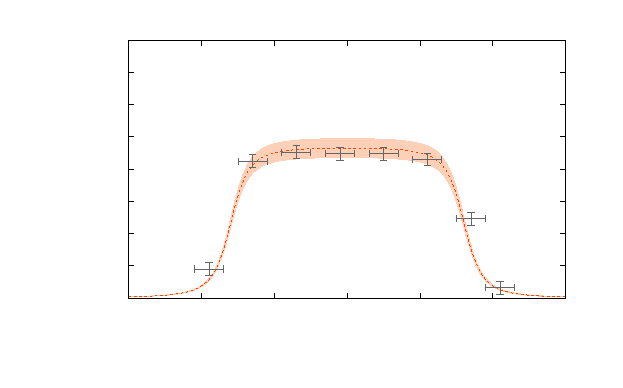
\includegraphics{camp-300-26}}%
    \gplfronttext
  \end{picture}%
\endgroup

	\caption{Camp magnètic al llarg de l'eix d'una bobina de 300 voltes, longitud \SI{16}{cm} i diàmetre \SI{2.6}{cm} per la que hi passa un corrent constant de \SI{1}{A}.}
	\label{fig:camp 300/26}
\end{figure}

A les \cref{fig:camp 300/33,fig:camp 75/26,fig:camp 150/26,fig:camp 300/26} hi ha representat el mòdul del camp magnètic al llarg de l'eix de les bobines mesurades durant l'experiment---calculat a partir de l'\cref{eq:camp bobina} i amb el corresponent marge d'incertesa--- aixì com els punts corresponents a les mesures realitzades

Tal i com es pot apreciar, al llarg de l'eix les mesures obtingudes s'ajusten molt bé a la prediccío teòrica. Això és d'esperar ja que a l'interior d'una bobina el camp és pràcticament constant. Als extrems, però, les dades experimentals no s'hi ajusten tant. Una explicació és que en  

\section{Conclusions}
En general els resultats obtinguts han estat satisfactoris. S'ha observat empíricament al llarg de tota la pràctica els fets que s'havien demostrat de manera teòrica. El camp magnètic al centre d'una espira disminueix a mesura que augmenta el radi d'aquesta i ho fa com $\frac{1}{R}$ amb $R$ el radi de l'espira. S'ha comprovat també empíricament l'augment lineal del camp al centre d'un conjunt d'espires amb la quantitat d'espires. Aquest últim fet ha estat provat per conjunts de $1$, $2$ i $3$ espires. Les observacions han portat també a concloure que el camp magnètic al centre d'una bobina augmenta en apropar-se al centre i és màxim en aquest. El fet que el camp magnètic creat per una bobina on hi circula una certa intensitat augmenta amb el nombre de voltes, ha estat provat també de manera satisfactòria. Finalment s'ha calculat empíricament la permeabilitat magnètica $\mu_{0}$ i s'ha obtingut una bona aproximació d'aquesta.






% Annexos
\addcontentsline{toc}{part}{Annexos}
\appendix
\titleformat{\chapter}[display]{\centering \bfseries \sffamily \LARGE}{\large \sf Annex \thechapter}{4pt}{}{}
\titlespacing{\chapter}{0pt}{*2}{*4}

\chapter{Annexos}
\section{Annex}
\todo{S'ha de decidir l'estructura dels annexos}
\begin{table}
	\centering
	\sffamily \small
	\caption{Mesures de la intensitat necessària per contrarrestar la força gravitatòria de cada massa}
	\label{tab:forca v intensitat (detall)}

	\todo[inline]{No sé com fer aquesta taula}

	\begin{tabular}{SSSSS}
		\toprule	
		\multicolumn{5}{c}{Massa (\si{mg})} \\
		{5} & {10} & {15} & {20} & {25} \\
		\midrule 
		2.62 & 3.70 & 4.47 & 5.10 & 6.05 \\
		2.55 & 3.40 & 4.46 & 5.29 & 5.99 \\
		2.65 & 3.58 & 4.63 & 5.33 & 5.94 \\
		2.62 & 3.64 & 4.42 & 5.07 & 5.40 \\
		2.60 & 3.71 & 4.50 & 5.10 & 5.21 \\
		2.57 & 3.68 & 4.48 & 5.11 & 5.63 \\
		\bottomrule
	\end{tabular}
\end{table}


\begin{table}
	\centering
	\sffamily
	\small
	\caption{Dades de la regressió lineal entre la força del fil de torsió i la rotació del dial}
	\label{tab:regressio forca-angle}

	\begin{tabular}{SS}
		\toprule
		{Mass (\si{mg})} & {Rotació (\si{\degree}) (\( {} \pm \SI{1}{\degree} \))} \\
		\midrule
		5 & 13 \\
		10 & 27 \\
		15 & 44 \\
		20 & 63 \\
		25 & 70 \\
		\bottomrule
	\end{tabular}
\end{table}

\begin{figure}
	\centering
	% GNUPLOT: LaTeX picture with Postscript
\begingroup
\sffamily \small
  \makeatletter
  \providecommand\color[2][]{%
    \GenericError{(gnuplot) \space\space\space\@spaces}{%
      Package color not loaded in conjunction with
      terminal option `colourtext'%
    }{See the gnuplot documentation for explanation.%
    }{Either use 'blacktext' in gnuplot or load the package
      color.sty in LaTeX.}%
    \renewcommand\color[2][]{}%
  }%
  \providecommand\includegraphics[2][]{%
    \GenericError{(gnuplot) \space\space\space\@spaces}{%
      Package graphicx or graphics not loaded%
    }{See the gnuplot documentation for explanation.%
    }{The gnuplot epslatex terminal needs graphicx.sty or graphics.sty.}%
    \renewcommand\includegraphics[2][]{}%
  }%
  \providecommand\rotatebox[2]{#2}%
  \@ifundefined{ifGPcolor}{%
    \newif\ifGPcolor
    \GPcolortrue
  }{}%
  \@ifundefined{ifGPblacktext}{%
    \newif\ifGPblacktext
    \GPblacktextfalse
  }{}%
  % define a \g@addto@macro without @ in the name:
  \let\gplgaddtomacro\g@addto@macro
  % define empty templates for all commands taking text:
  \gdef\gplbacktext{}%
  \gdef\gplfronttext{}%
  \makeatother
  \ifGPblacktext
    % no textcolor at all
    \def\colorrgb#1{}%
    \def\colorgray#1{}%
  \else
    % gray or color?
    \ifGPcolor
      \def\colorrgb#1{\color[rgb]{#1}}%
      \def\colorgray#1{\color[gray]{#1}}%
      \expandafter\def\csname LTw\endcsname{\color{white}}%
      \expandafter\def\csname LTb\endcsname{\color{black}}%
      \expandafter\def\csname LTa\endcsname{\color{black}}%
      \expandafter\def\csname LT0\endcsname{\color[rgb]{1,0,0}}%
      \expandafter\def\csname LT1\endcsname{\color[rgb]{0,1,0}}%
      \expandafter\def\csname LT2\endcsname{\color[rgb]{0,0,1}}%
      \expandafter\def\csname LT3\endcsname{\color[rgb]{1,0,1}}%
      \expandafter\def\csname LT4\endcsname{\color[rgb]{0,1,1}}%
      \expandafter\def\csname LT5\endcsname{\color[rgb]{1,1,0}}%
      \expandafter\def\csname LT6\endcsname{\color[rgb]{0,0,0}}%
      \expandafter\def\csname LT7\endcsname{\color[rgb]{1,0.3,0}}%
      \expandafter\def\csname LT8\endcsname{\color[rgb]{0.5,0.5,0.5}}%
    \else
      % gray
      \def\colorrgb#1{\color{black}}%
      \def\colorgray#1{\color[gray]{#1}}%
      \expandafter\def\csname LTw\endcsname{\color{white}}%
      \expandafter\def\csname LTb\endcsname{\color{black}}%
      \expandafter\def\csname LTa\endcsname{\color{black}}%
      \expandafter\def\csname LT0\endcsname{\color{black}}%
      \expandafter\def\csname LT1\endcsname{\color{black}}%
      \expandafter\def\csname LT2\endcsname{\color{black}}%
      \expandafter\def\csname LT3\endcsname{\color{black}}%
      \expandafter\def\csname LT4\endcsname{\color{black}}%
      \expandafter\def\csname LT5\endcsname{\color{black}}%
      \expandafter\def\csname LT6\endcsname{\color{black}}%
      \expandafter\def\csname LT7\endcsname{\color{black}}%
      \expandafter\def\csname LT8\endcsname{\color{black}}%
    \fi
  \fi
    \setlength{\unitlength}{0.0500bp}%
    \ifx\gptboxheight\undefined%
      \newlength{\gptboxheight}%
      \newlength{\gptboxwidth}%
      \newsavebox{\gptboxtext}%
    \fi%
    \setlength{\fboxrule}{0.5pt}%
    \setlength{\fboxsep}{1pt}%
\begin{picture}(5668.00,3400.00)%
    \gplgaddtomacro\gplbacktext{%
      \csname LTb\endcsname%%
      \put(1078,704){\makebox(0,0)[r]{\strut{}\num{0}}}%
      \put(1078,1117){\makebox(0,0)[r]{\strut{}\num{0.05}}}%
      \put(1078,1529){\makebox(0,0)[r]{\strut{}\num{0.1}}}%
      \put(1078,1942){\makebox(0,0)[r]{\strut{}\num{0.15}}}%
      \put(1078,2354){\makebox(0,0)[r]{\strut{}\num{0.2}}}%
      \put(1078,2767){\makebox(0,0)[r]{\strut{}\num{0.25}}}%
      \put(1078,3179){\makebox(0,0)[r]{\strut{}\num{0.3}}}%
      \put(1210,484){\makebox(0,0){\strut{}\num{10}}}%
      \put(1790,484){\makebox(0,0){\strut{}\num{20}}}%
      \put(2370,484){\makebox(0,0){\strut{}\num{30}}}%
      \put(2950,484){\makebox(0,0){\strut{}\num{40}}}%
      \put(3531,484){\makebox(0,0){\strut{}\num{50}}}%
      \put(4111,484){\makebox(0,0){\strut{}\num{60}}}%
      \put(4691,484){\makebox(0,0){\strut{}\num{70}}}%
      \put(5271,484){\makebox(0,0){\strut{}\num{80}}}%
    }%
    \gplgaddtomacro\gplfronttext{%
      \csname LTb\endcsname%%
      \put(198,1941){\rotatebox{-270}{\makebox(0,0){\strut{}$\mathsf{F \ (\si{mN})}$}}}%
      \put(3240,154){\makebox(0,0){\strut{}$\mathsf{\theta \ (\si{\degree})}$}}%
    }%
    \gplbacktext
    \put(0,0){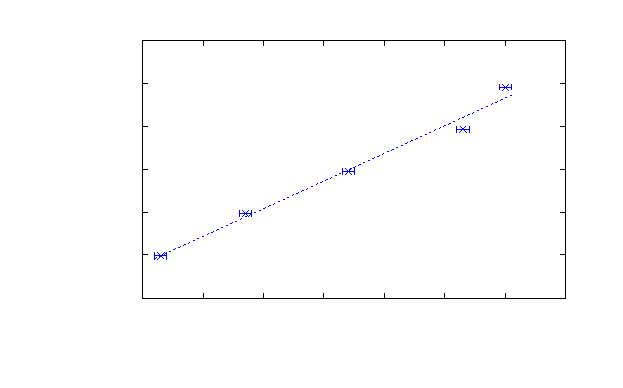
\includegraphics{forca-rotacio}}%
    \gplfronttext
  \end{picture}%
\endgroup

	\caption{Força en funció de la rotació del dial}
	\label{fig:força v rotacio}
\end{figure}



\end{document}

